\documentclass[a4paper,12pt]{article}
\usepackage{graphicx}       %LaTeX package to import graphics

\usepackage[T1]{fontenc}
\usepackage[italian]{babel}

\usepackage{subcaption}

\usepackage{hyphenat}
\usepackage{array}
\usepackage{booktabs}       % Per linee orizzontali migliori
\usepackage{caption}        % Per personalizzare le didascalie<
\usepackage{multirow}       % Per combinare celle nelle colonne
\usepackage{hyperref}

\usepackage{bm} 

\usepackage{amsmath}        % Per migliorare l'aspetto delle formule

\usepackage{todonotes}      % mettere le note dentro il documento

\usepackage{siunitx}        % Per formattare le unità di misura
\usepackage{gensymb}        % Simboli come °
\usepackage{xfrac}          % per fare le frazioni inclinate

\usepackage{pdfpages}

\usepackage{import}
\usepackage{frontespizio}

\usepackage{placeins}       %per non far andare le immagini al di fuori delle sezioni utilizzare il comando: \FloatBarrier non far superare le immagini quel punto

\usepackage{adjustbox}      % per dimensionare le immagini in modo automatico


\begin{document}

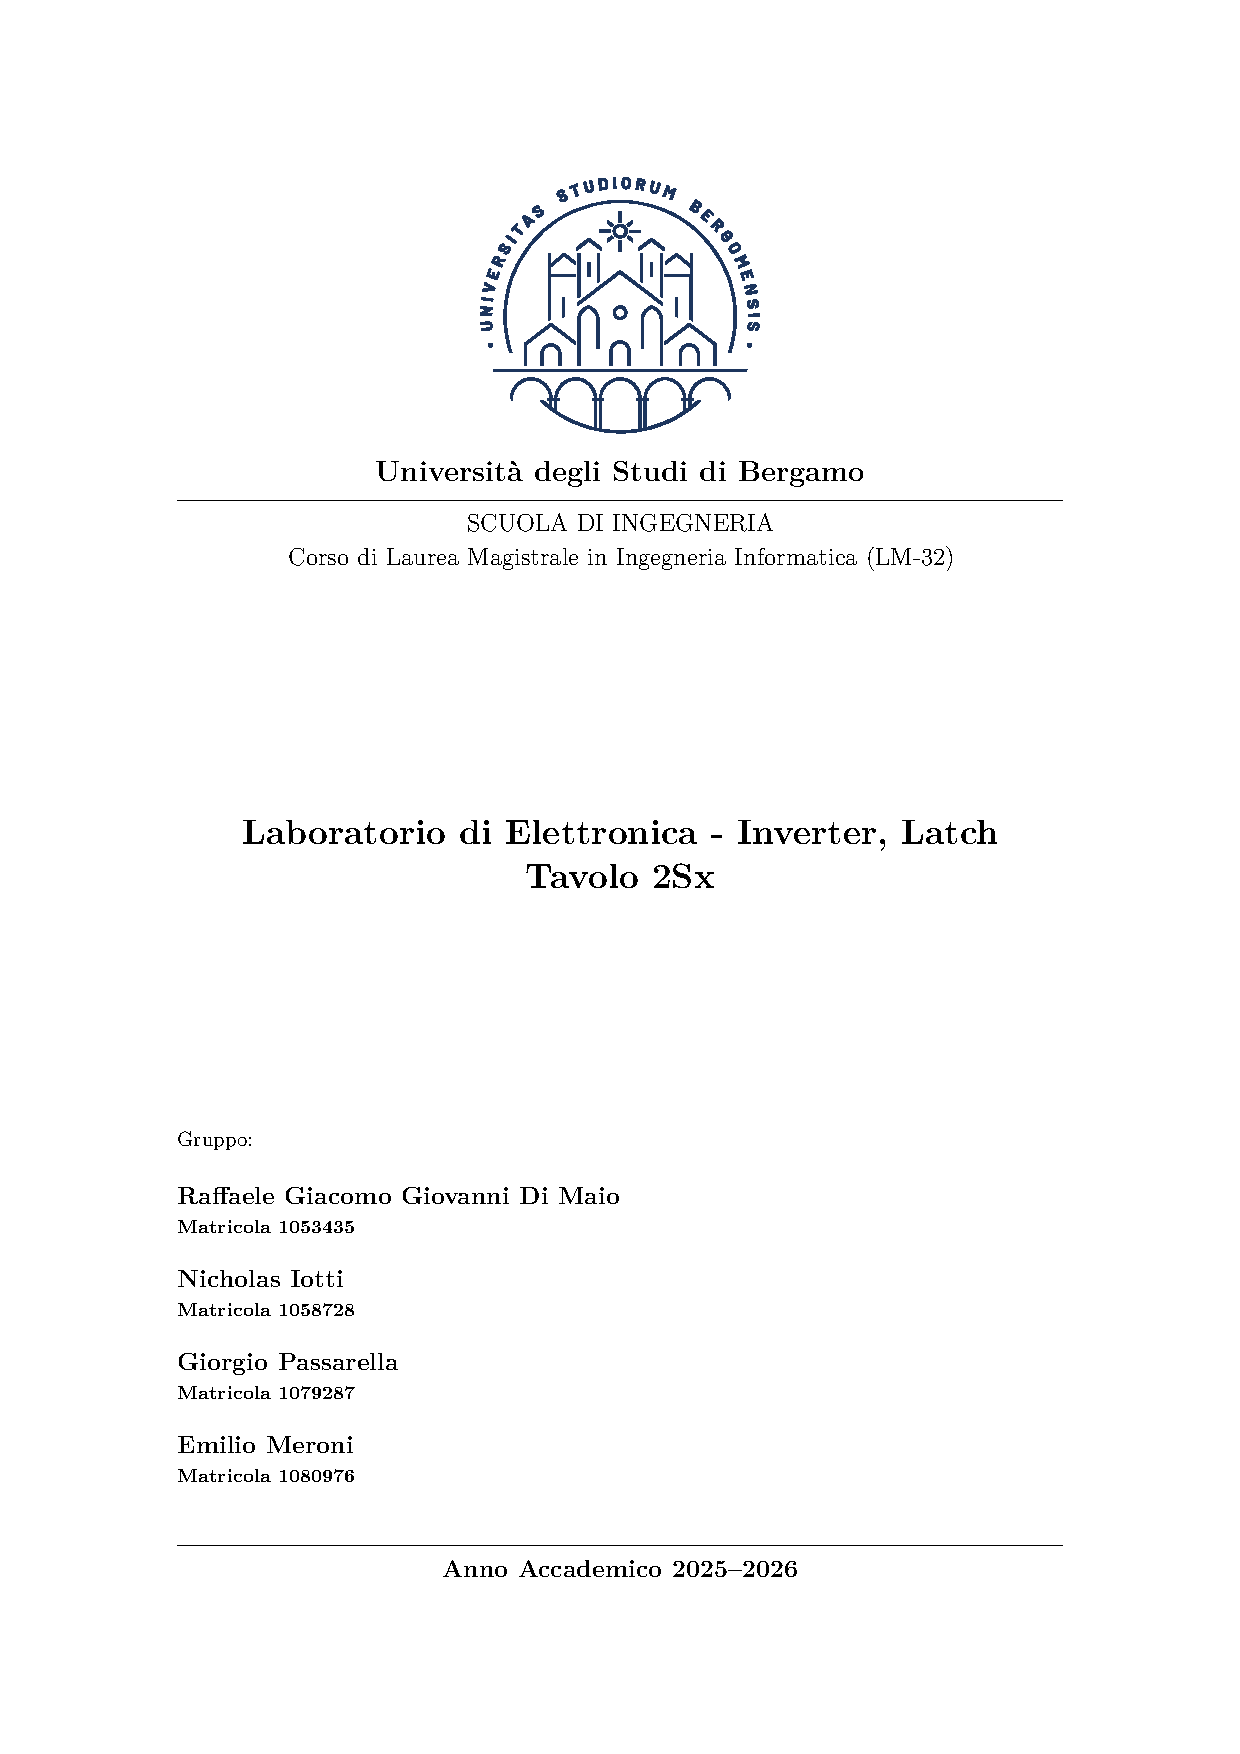
\includepdf{./frontespizio/frontespizio.pdf}

\section*{Circuiti Digitali}

Nei circuiti digitali, a differenza di quelli analogici, il segnale è discretizzato sia nei tempi che nelle ampiezze (figura \ref{fig:digitali-differenza}), in particolare esso può assumere dei valori alti $V_H$ o bassi $V_L$, tipicamente $5\,V$ e $0\,V$.

\begin{figure}[h]
	\centering
	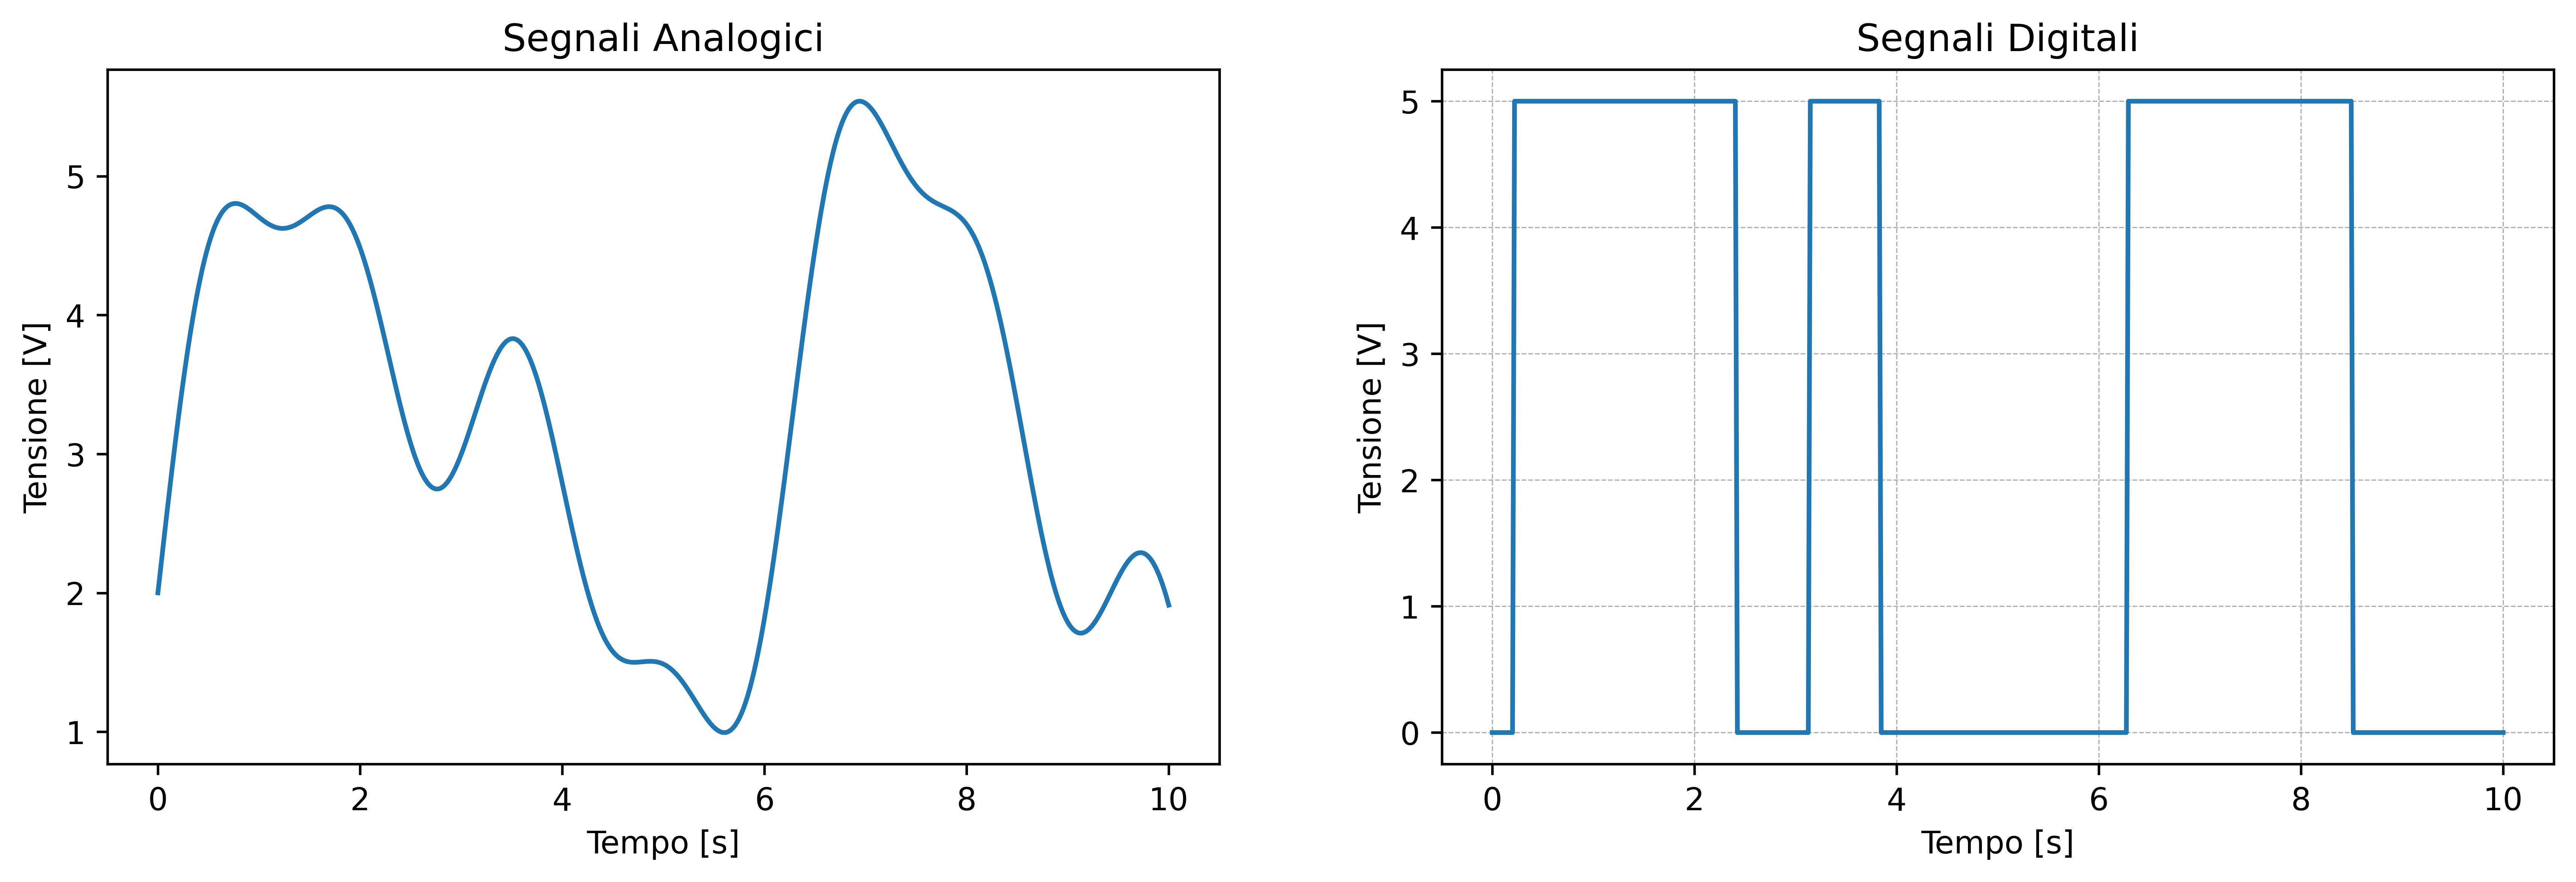
\includegraphics[width=1\linewidth]{immagini/circuiti-digitali/differenza-circuiti-analogici-digitali.png}
	\caption{Differenza tra i segnali analogici e digitali.}
	\label{fig:digitali-differenza}
\end{figure}

I circuiti digitali possono lavorare con due tipologie di logiche:
\begin{itemize}
	\item \textbf{Logica Combinatoria}, l'uscita dipende sono dal valore degli ingressi in quell'istante;
	\item \textbf{Logica Sequenziale}, in questo caso si hanno degli stati interni e quindi per determinare l'uscita non basta conoscere il valore degli ingressi.
\end{itemize}

\subsection*{Porte Logiche}
Di seguito si riportano alcune tabelle della verità delle porte logiche più semplici:


\begin{table}[h]
	\parbox{.30\linewidth}{
		\centering
		\setlength{\tabcolsep}{10pt}
		\begin{tabular}{cc|c}
			\textbf{A} & \textbf{B} & \textbf{Q} \\
			\midrule
			0 & 0 & 0 \\
			0 & 1 & 0 \\
			1 & 0 & 0 \\
			1 & 1 & 1 \\
		\end{tabular}
		\caption{AND o prodotto logico}
	}
	\hfil
	\parbox{.30\linewidth}{
		\centering
		\setlength{\tabcolsep}{10pt}
		\begin{tabular}{cc|c}
			\textbf{A} & \textbf{B} & \textbf{Q} \\
			\midrule
			0 & 0 & 0 \\
			0 & 1 & 1 \\
			1 & 0 & 1 \\
			1 & 1 & 1 \\
		\end{tabular}
		\caption{OR o somma logica}
	}
	\hfil
	\parbox{.30\linewidth}{
		\centering
		\setlength{\tabcolsep}{10pt}
		\begin{tabular}{c|c}
			\textbf{A} & \textbf{Q} \\
			\midrule
			0 & 1 \\
			1 & 0 \\
		\end{tabular}
		\caption{Inverter}
		\label{tab:inverter-tabella-verita}
	}
\end{table}

\subsection*{Teorema di Demorgan e mappa di Karnaugh}
Grazie al teorema di Demorgan, che mette in relazione l'operazione AND con l'operazione OR, e alle mappe di Karnaugh si possono semplificare i circuiti logici. In particolare, le mappe di Karnaugh esprimono una qualsiasi tabella della verità come somma di prodotti (oppure come prodotti di somme) e successivamente sfruttando il teorema di Demorgan il quale dice che:
\begin{align*}
	\overline{A + B} = \overline{A} \cdot \overline{B}\\
	\overline{A \cdot B} = \overline{A} + \overline{B}
\end{align*}
Ricaviamo che qualsiasi funzione logica può essere riscritta utilizzando solo porte logiche NAND (oppure NOR). 

\section*{Inverter CMOS}
L'inverter è un circuito digitale in cui l'uscita si trova al livello opposto dell'ingresso tabella \ref{tab:inverter-tabella-verita}. Per testarne il funzionamento è stato realizzato il circuito in \autoref{fig:inverterStatica}:

\begin{figure}[h]
	\centering
	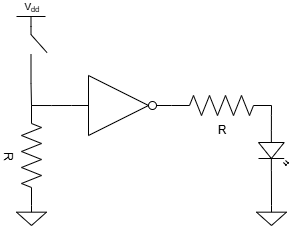
\includegraphics[width=0.4\linewidth]{immagini/inverter/circuitoLogico1Led.png}
	\caption{Schematico inverter.}
	\label{fig:inverterStatica}
\end{figure}


\noindent Si è utilizzato il circuito integrato \textbf{CB4069}, il quale è dotato di 14 pin, \autoref{fig:inverter-package}, il quale presenta 6 inverter.

\begin{figure}[h]
	\centering
	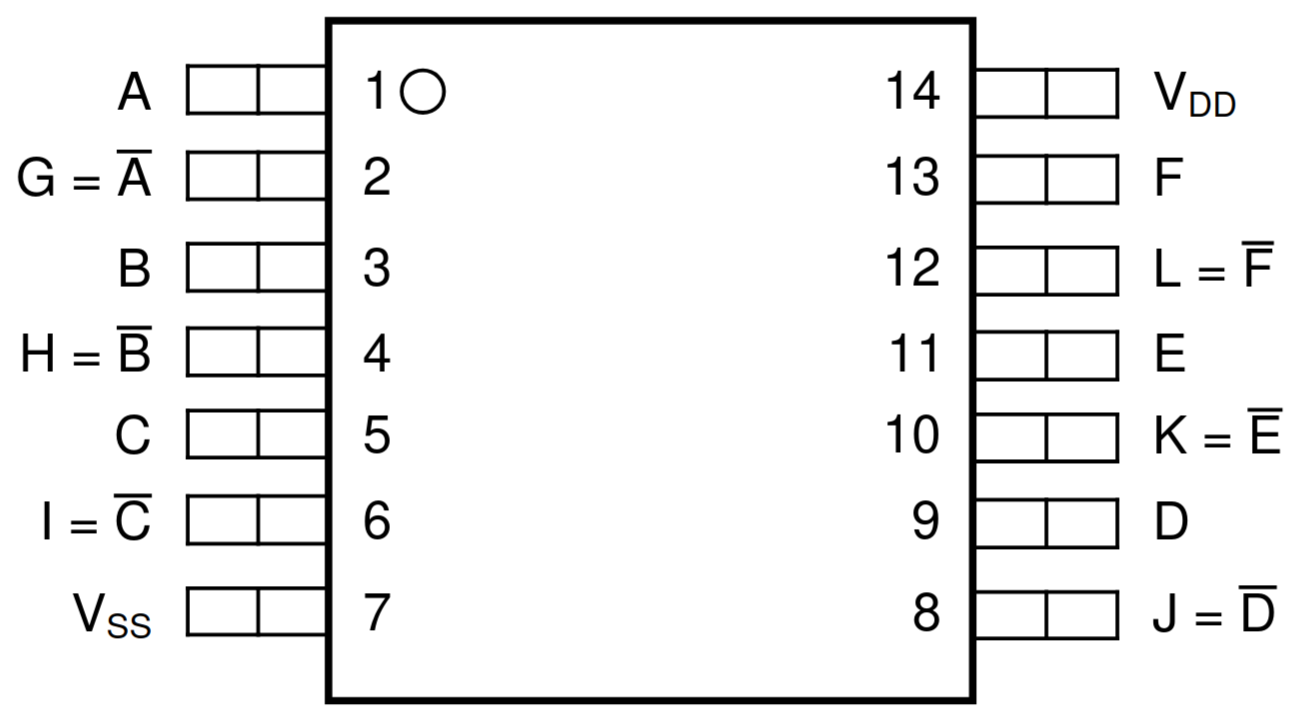
\includegraphics[width=0.3\linewidth]{immagini/inverter/package-inverter.png}
	\caption{Package Inverter.}
	\label{fig:inverter-package}
\end{figure}


È stata impostata una $V_{DD}$ di $5\,\mathrm{V}$ con l’obiettivo di verificare la caratteristica statica dell’inverter.
Per farlo, è stato forzato uno stato logico 0 o 1 all’ingresso dell’inverter e in uscita è stata posta una resistenza con in serie un diodo LED, in modo che, con uscita logica 1, il LED risulti acceso e con uscita logica 0 risulti spento come mostrato in \autoref{fig:statica}.


\begin{figure}[h]
	\centering
	\begin{subfigure}[b]{0.40\textwidth}
		\centering
		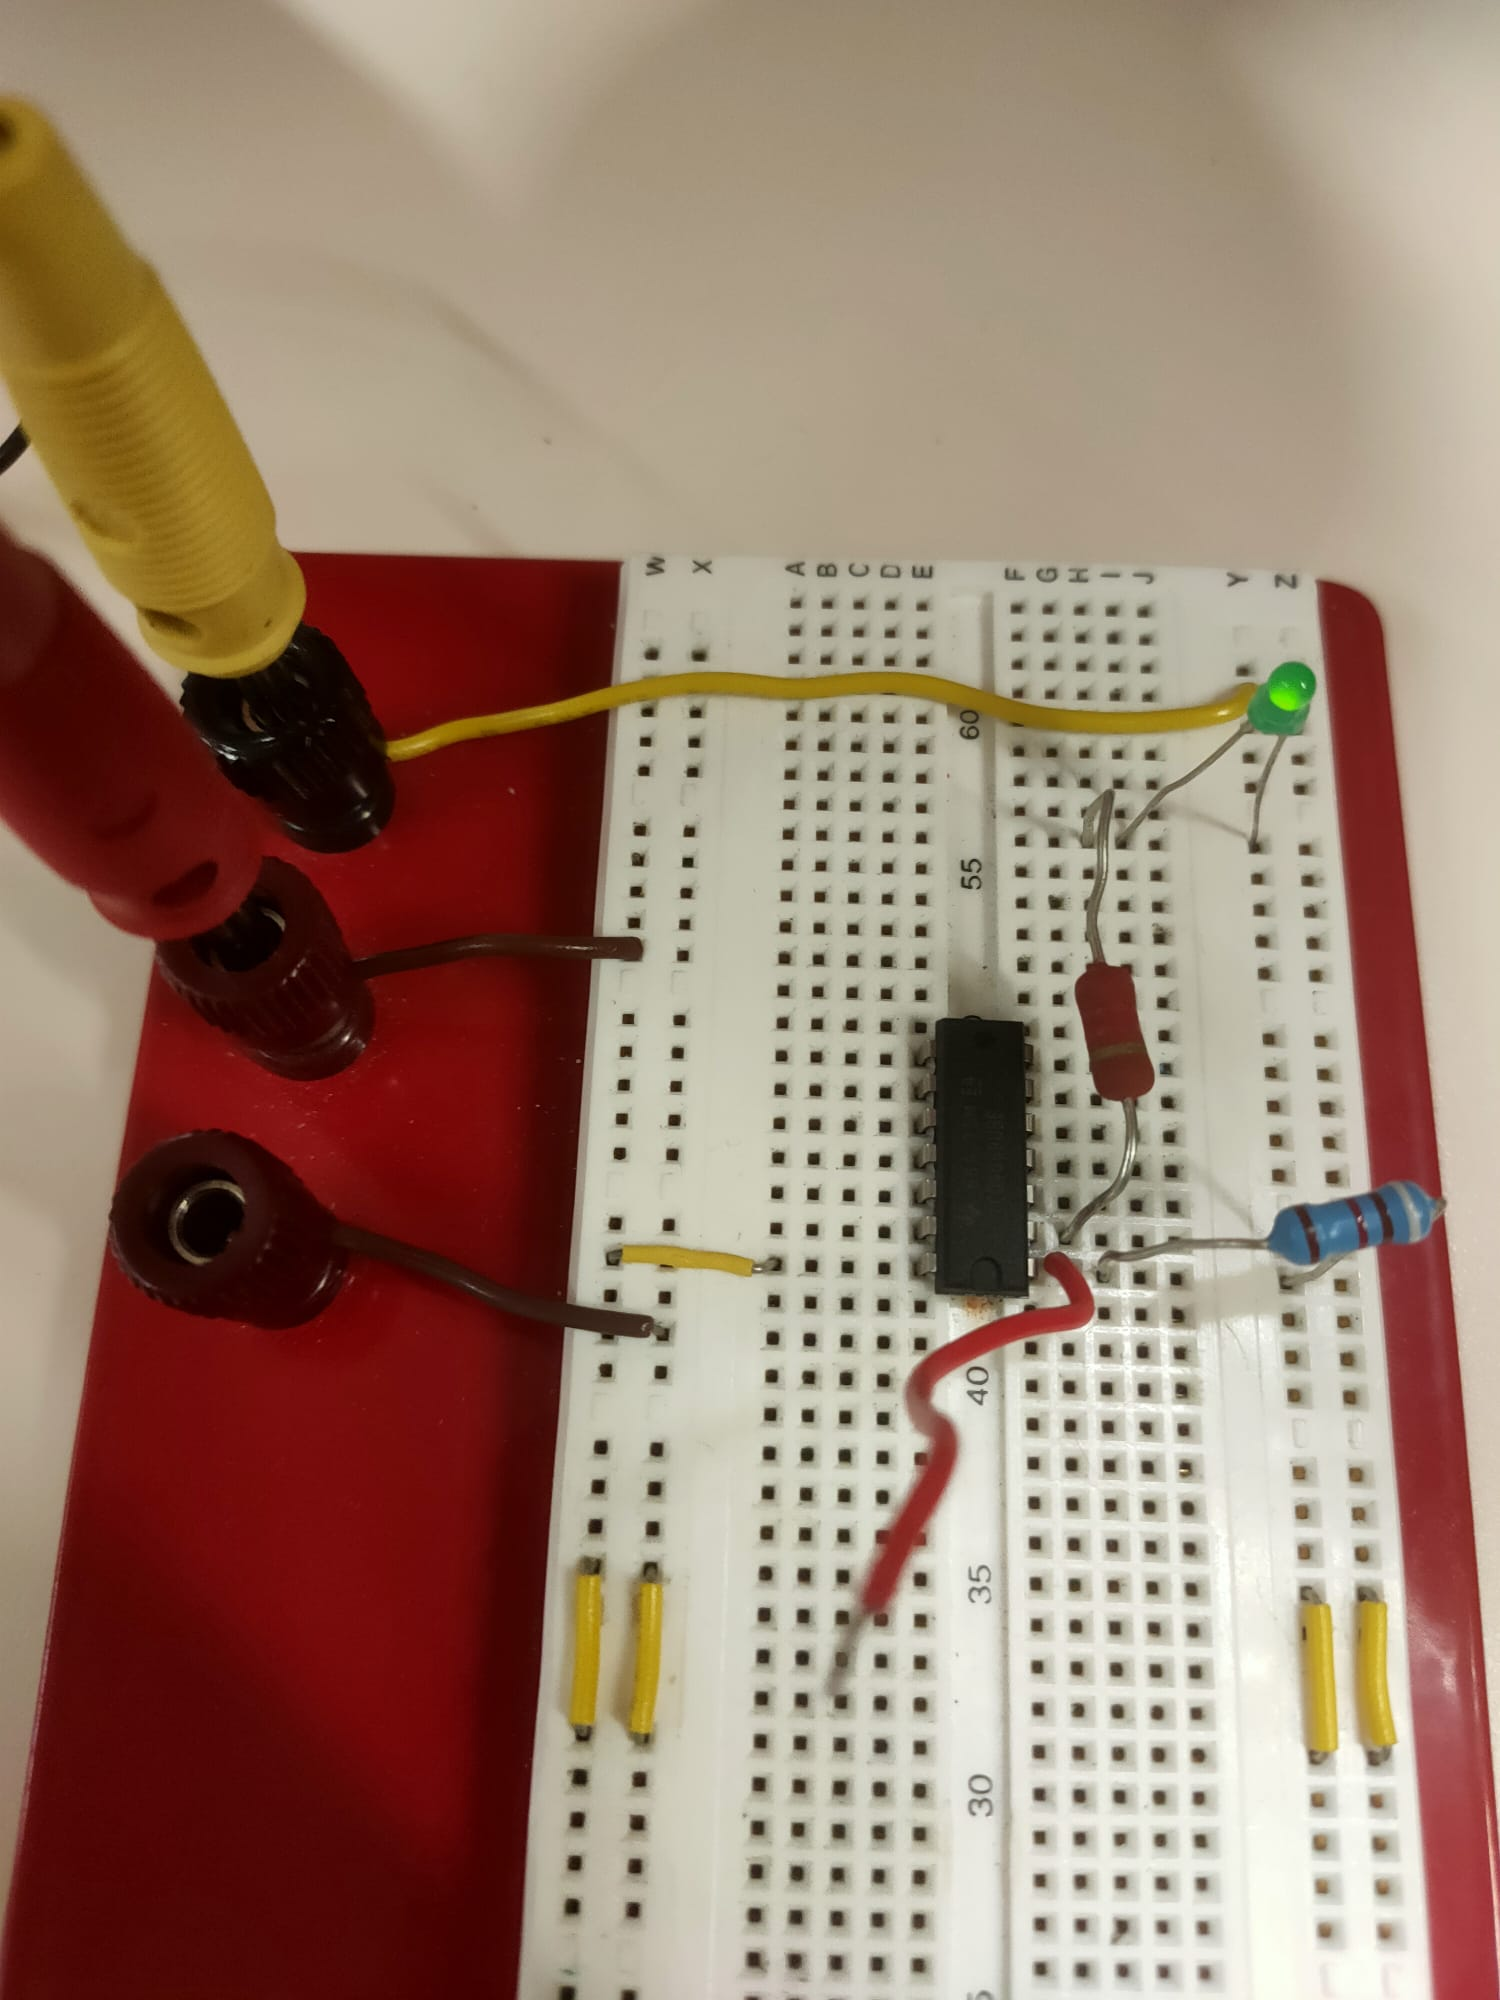
\includegraphics[width=\textwidth]{immagini/inverter/on.png}
		\caption{Uscita logica 1 - LED acceso}
		\label{fig:led_on}
	\end{subfigure}
	\quad
	\begin{subfigure}[b]{0.40\textwidth}
		\centering
		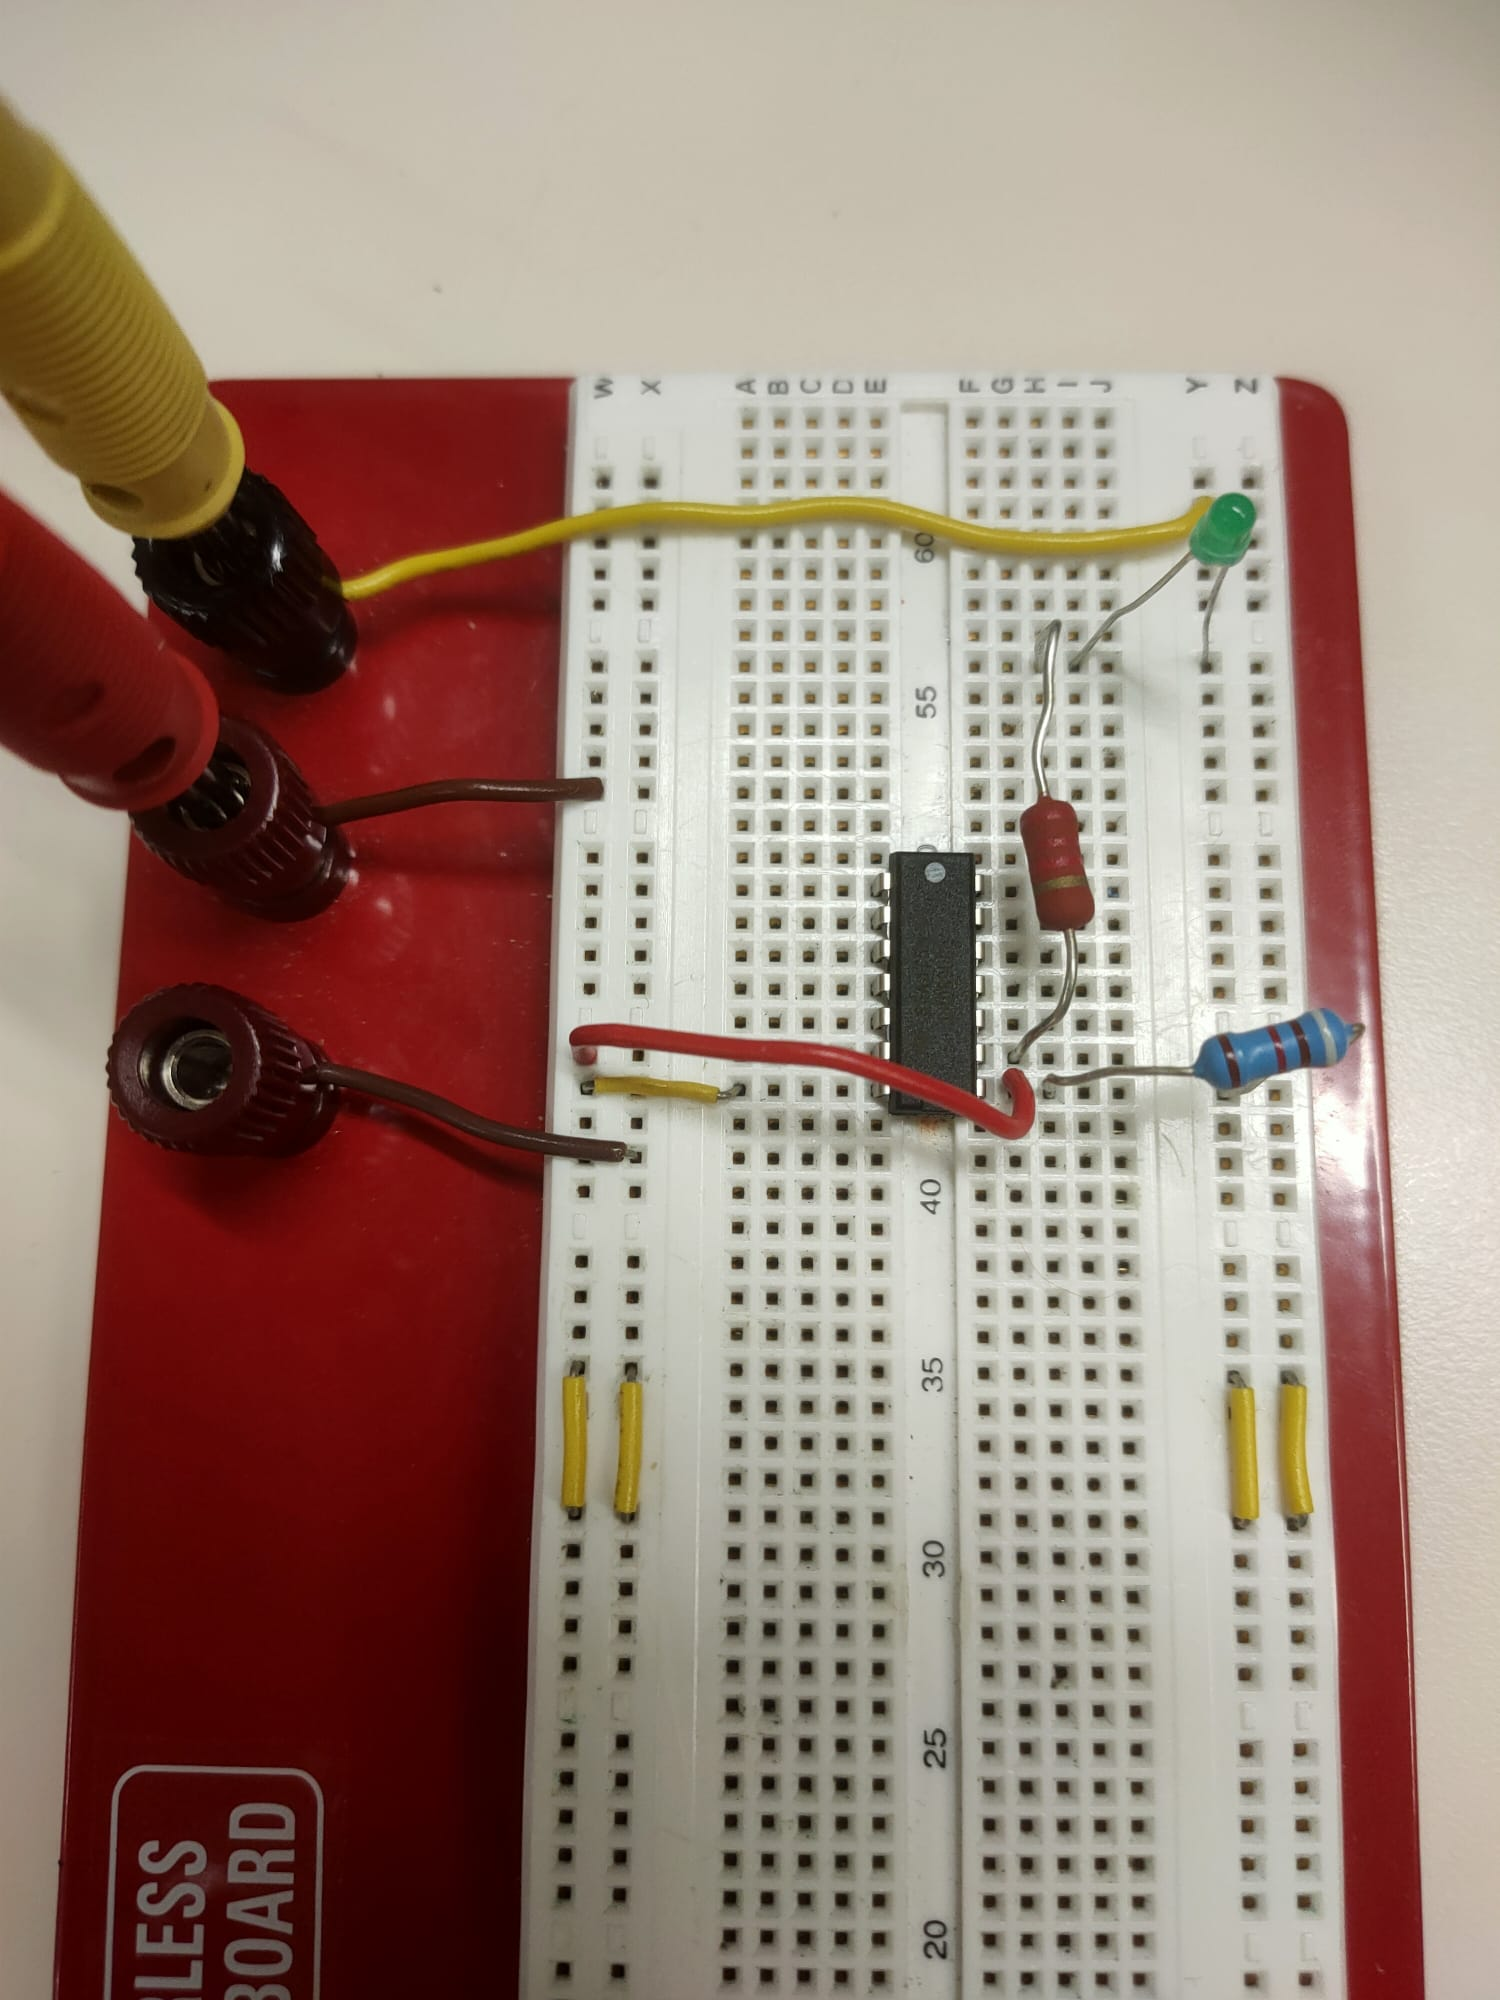
\includegraphics[width=\textwidth]{immagini/inverter/off.png}
		\caption{Uscita logica 0 - LED spento}
		\label{fig:led_off}
	\end{subfigure}
	\caption{Verifica della caratteristica statica dell'inverter tramite LED}
	\label{fig:statica}
\end{figure}


Successivamente andando a modificare il circuito come in \autoref{fig:inverterDinamica}, è stato possibile verificare la caratteristica dinamica collegando l’ingresso del circuito a un generatore di forme d’onda che fornisce un segnale ad onda quadra con un’ampiezza di $5\,\mathrm{V}_{pp}$ e un offset di $2.5\,\mathrm{V}$, simulando la commutazione di un bit tra 0 e 1, per osservare la negazione in uscita.

\begin{figure}[h]
	\centering
	\begin{subfigure}[b]{0.45\textwidth}
		\centering
		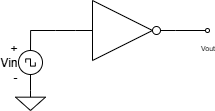
\includegraphics[width=\linewidth]{immagini/inverter/circuitoLogico1NoLed.png}
		\caption{Schematico dell'inverter per la verifica della caratteristica dinamica.}
		\label{fig:inverterDinamica}
	\end{subfigure}
	\hfill
	\begin{subfigure}[b]{0.45\textwidth}
		\centering
		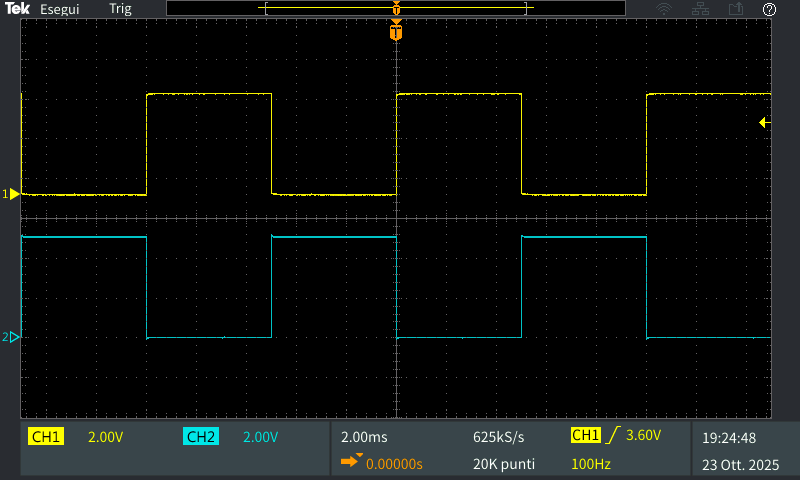
\includegraphics[width=\linewidth]{immagini/inverter/TEK00099.PNG}
		\caption{Caratteristica dinamica dell'inverter.}
		\label{grafico}
	\end{subfigure}
	\caption{Verifica della caratteristica dinamica dell'inverter: a sinistra lo schema del circuito, a destra la risposta osservata all'oscilloscopio.}
	\label{fig:inverterDinamica}
\end{figure}

Infine, sono stati calcolati il tempo di salita, il tempo di discesa e il ritardo di propagazione dell’inverter.
In \autoref{fig:ritardo_propagazione} è riportata la misura del ritardo di propagazione, pari a circa \SI{23.6}{\nano\second}.
Le \autoref{fig:salita} e \autoref{fig:discesa} mostrano rispettivamente i fronti di salita e discesa del segnale in uscita, con tempi pari a circa \SI{30}{\nano\second} e \SI{20}{\nano\second}.


\begin{figure}[h]
	\centering
	\begin{subfigure}[b]{0.48\textwidth}
		\centering
		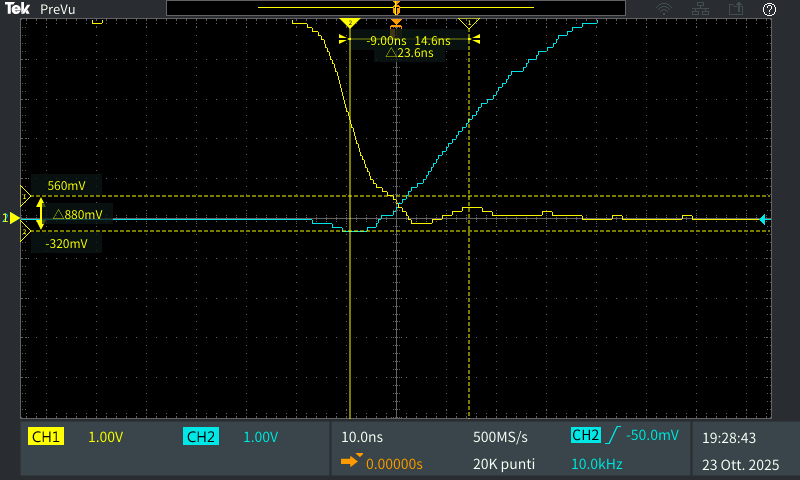
\includegraphics[width=\linewidth]{immagini/inverter/TEK00100.PNG}
		\caption{Ritardo di propagazione (\SI{23.6}{\nano\second}).}
		\label{fig:ritardo_propagazione}
	\end{subfigure}
	\hfill
	\begin{subfigure}[b]{0.48\textwidth}
		\centering
		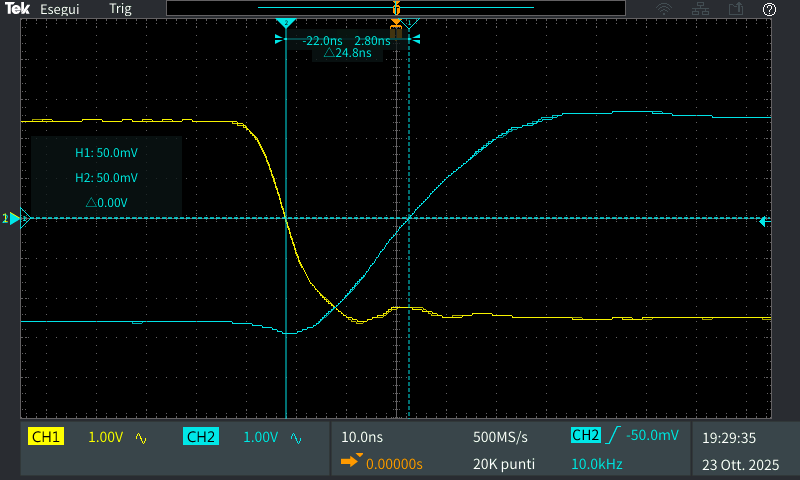
\includegraphics[width=\linewidth]{immagini/inverter/TEK00101.PNG}
		\caption{Transizioni complete.}
		\label{fig:transizioni_complete}
	\end{subfigure}
	\\[1em]
	\begin{subfigure}[b]{0.48\textwidth}
		\centering
		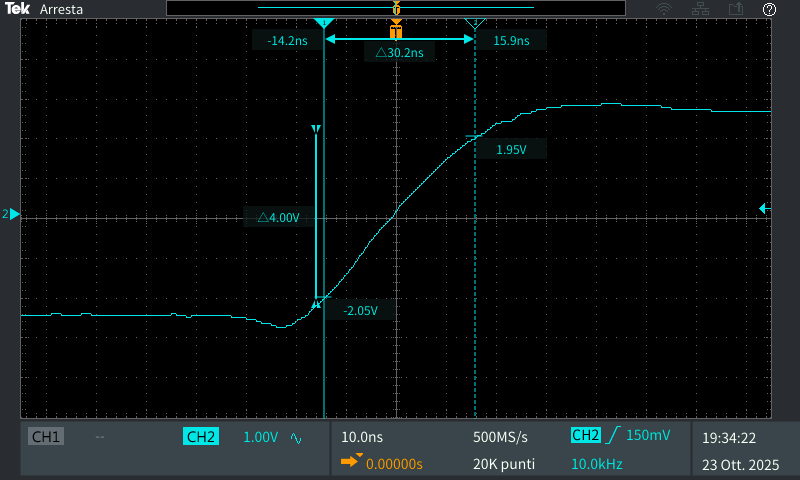
\includegraphics[width=\linewidth]{immagini/inverter/TEK00102.PNG}
		\caption{Tempo di salita (\SI{30}{\nano\second}).}
		\label{fig:salita}
	\end{subfigure}
	\hfill
	\begin{subfigure}[b]{0.48\textwidth}
		\centering
		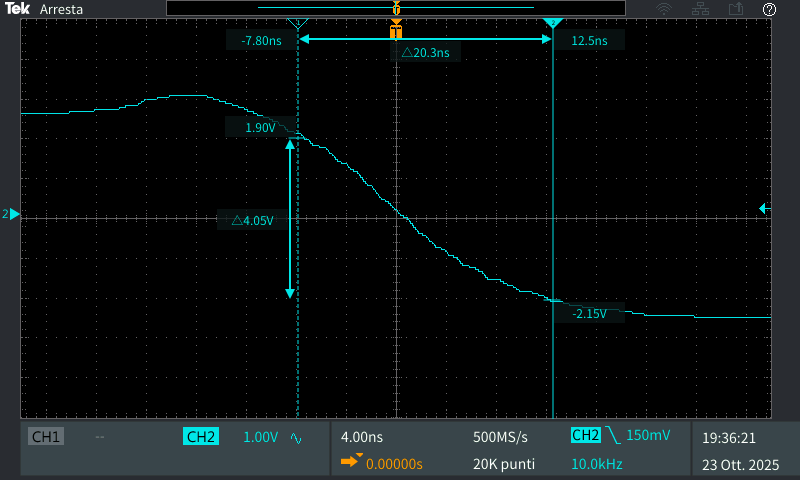
\includegraphics[width=\linewidth]{immagini/inverter/TEK00103.PNG}
		\caption{Tempo di discesa (\SI{20}{\nano\second}).}
		\label{fig:discesa}
	\end{subfigure}
	\caption{Misure sperimentali della caratteristica dinamica dell'inverter CMOS.}
	\label{fig:dinamica_misure}
\end{figure}

\FloatBarrier

\section*{Latch}

Il latch rappresenta una cella di memoria elementare, in grado di mantenere lo stato logico impostato anche dopo la rimozione del segnale di ingresso.
Il principio di funzionamento è caratterizzato dall’impiego di due inverter collegati in cascata e retroazionati, come mostrato nello schema in \autoref{fig:latch_schema}.

\begin{figure}[h]
	\centering
	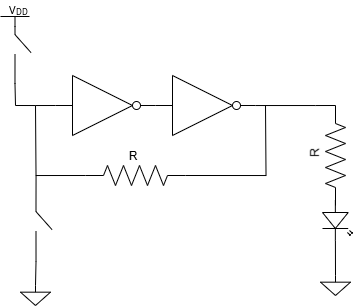
\includegraphics[width=0.5\linewidth]{immagini/latch/Latch.png}
	\caption{Schema circuitale del latch.}
	\label{fig:latch_schema}
\end{figure}

Quando viene applicato un livello logico 1 all’ingresso del primo inverter, la sua uscita assume valore logico 0, che a sua volta viene invertito dal secondo stadio, restituendo un livello logico 1.
Questo valore viene quindi mantenuto grazie all’anello di retroazione, che stabilizza il circuito nello stato logico impostato.
Un comportamento analogo si verifica quando viene applicato un livello logico 0: l’uscita del secondo inverter rimane a 0 fino a quando non interviene una nuova scrittura.
Per consentire la scrittura di uno stato logico, il circuito è stato dotato di due pulsanti:
uno collegato alla tensione di alimentazione $V_{DD}$ per impostare un livello logico alto, e uno collegato a massa per impostare un livello logico basso.
L’uscita è stata collegata a un LED per rendere visibile lo stato memorizzato: come mostrato in \autoref{fig:latch_onoff}, quando l’uscita è a livello logico 1 il LED risulta acceso, mentre con livello logico 0 rimane spento.

\begin{figure}[h]
	\centering
	\begin{subfigure}[b]{0.45\textwidth}
		\centering
		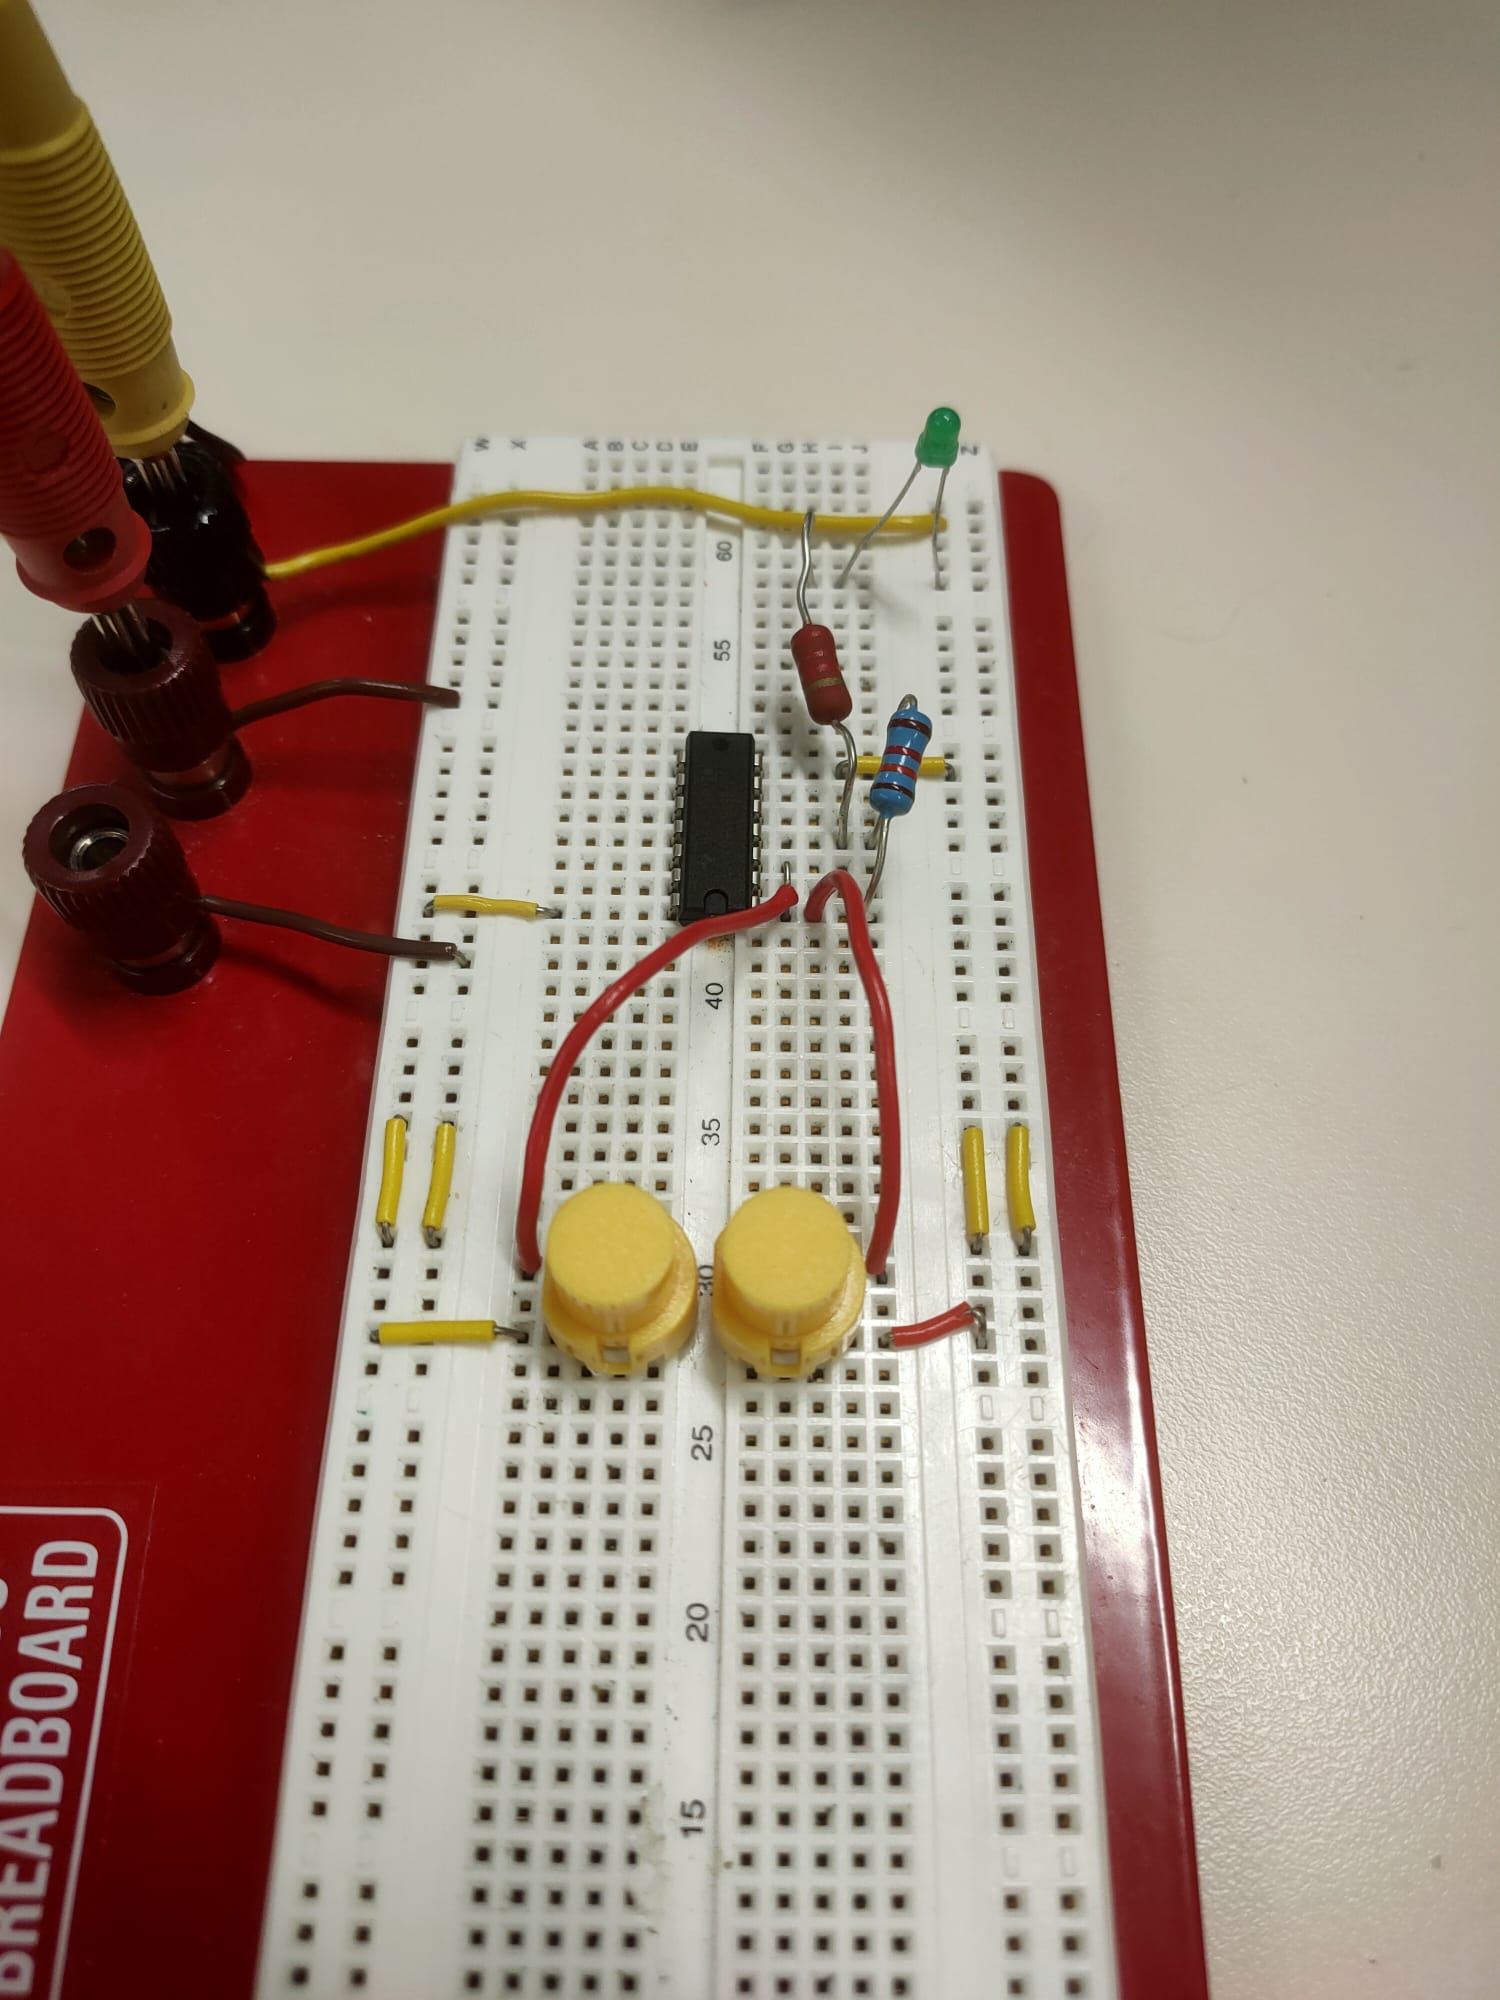
\includegraphics[width=\linewidth]{immagini/latch/off.png}
		\caption{Uscita logica 0, LED spento.}
	\end{subfigure}
	\quad
	\begin{subfigure}[b]{0.45\textwidth}
		\centering
		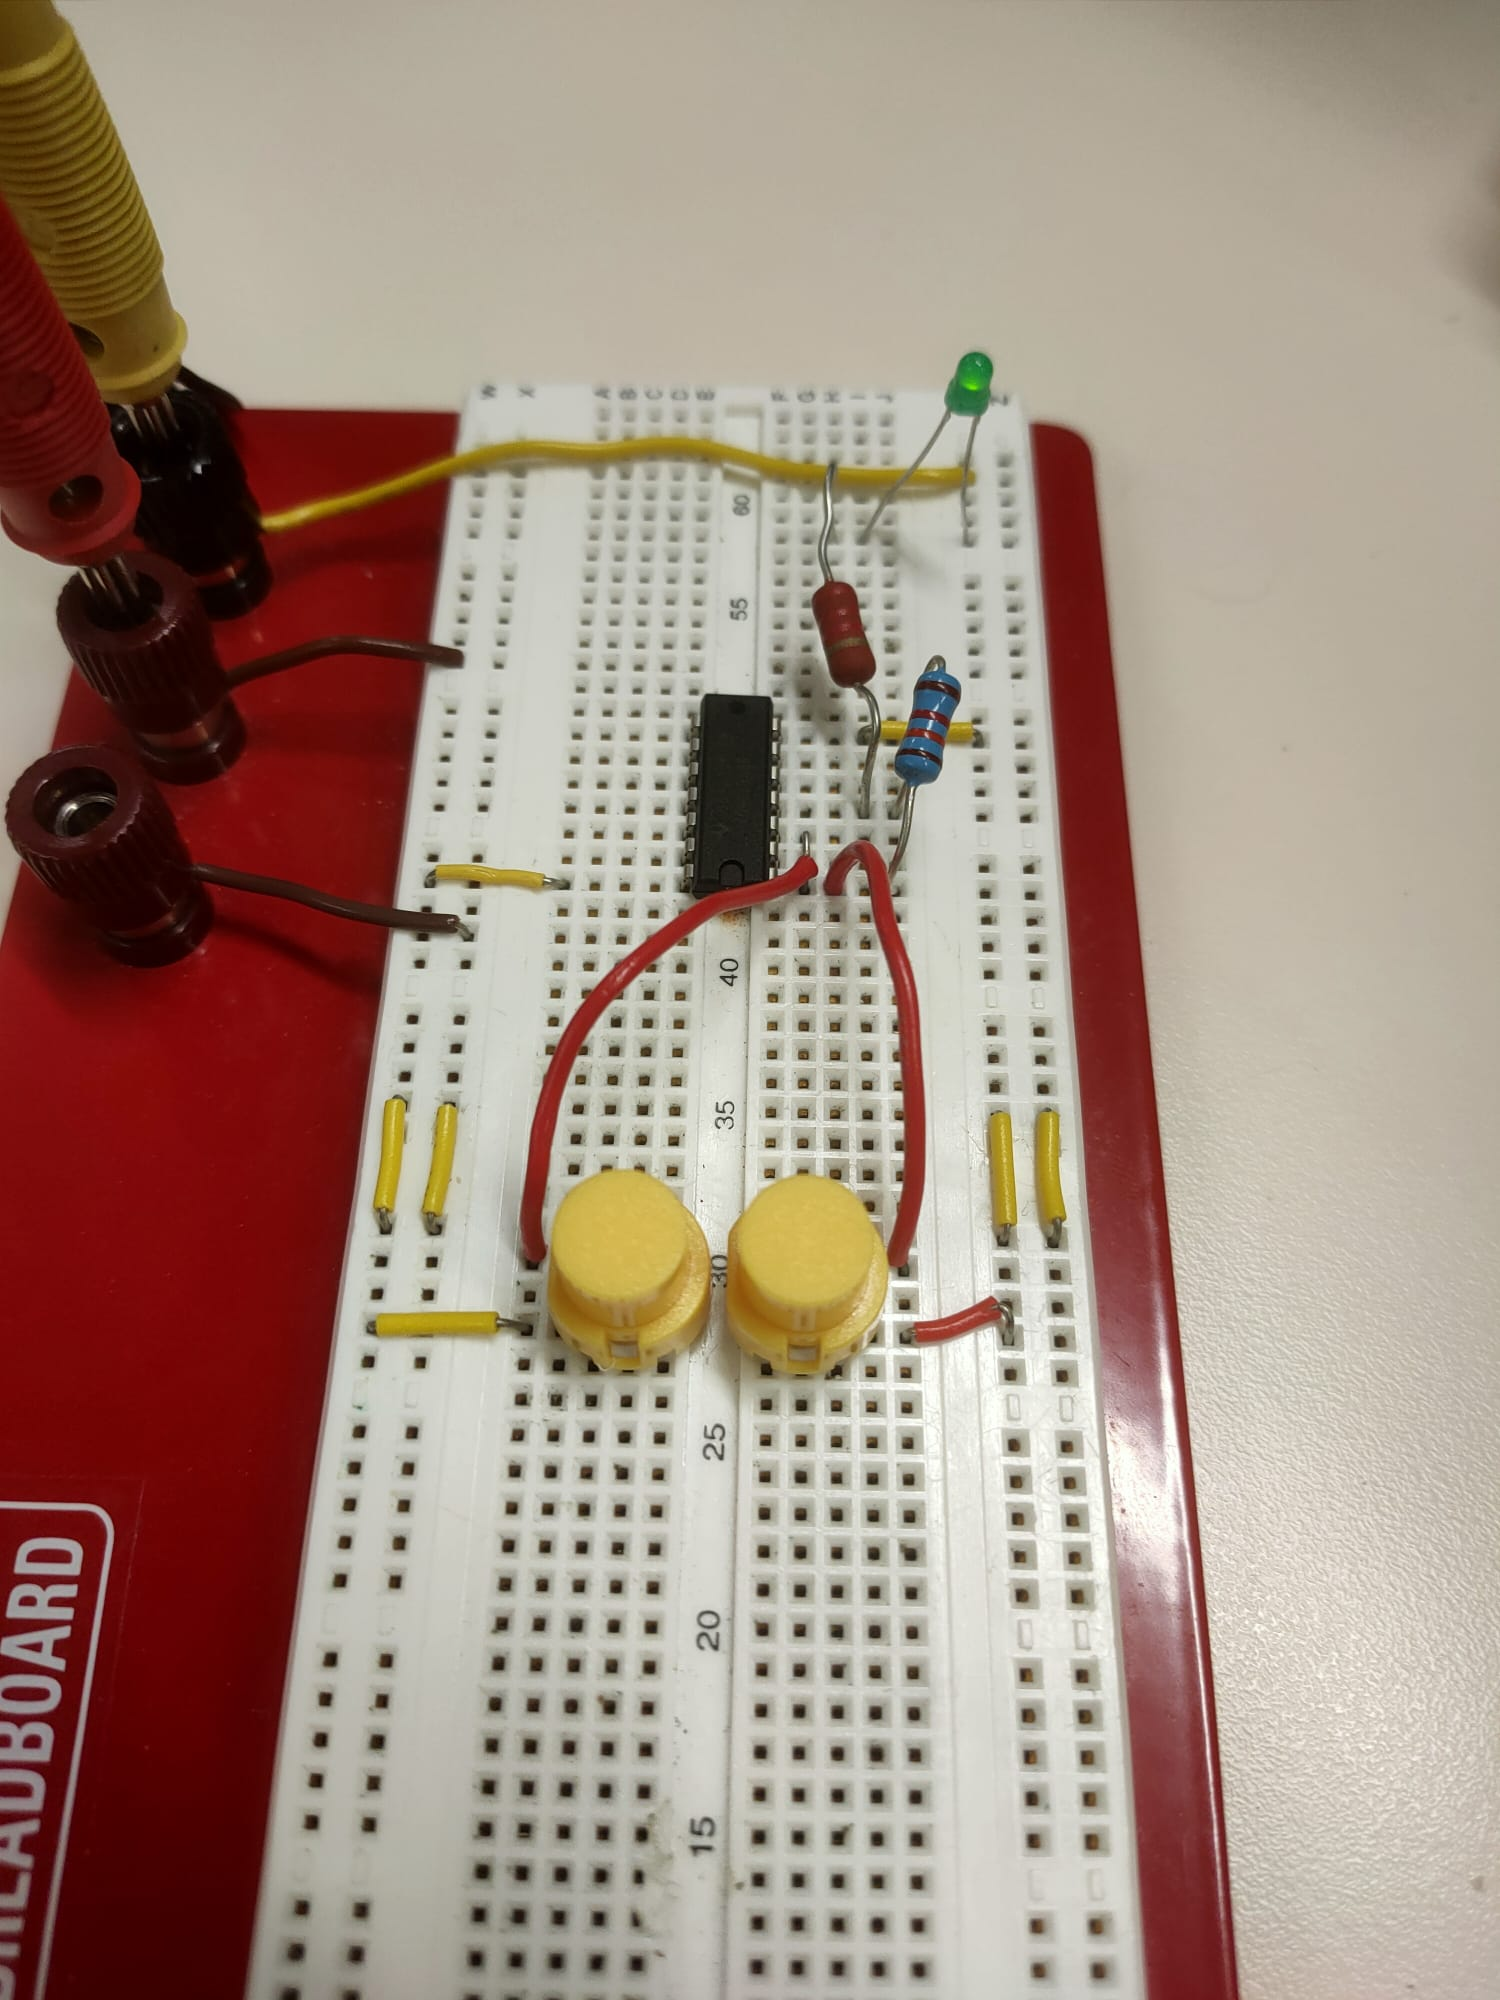
\includegraphics[width=\linewidth]{immagini/latch/on.png}
		\caption{Uscita logica 1, LED acceso.}
	\end{subfigure}
	\caption{Stati logici  dal latch.}
	\label{fig:latch_onoff}
\end{figure}


\FloatBarrier

\section*{Ring Oscillator}
Il Ring Oscillator, figura \ref{fig:ring-oscillator-schematico}, è un circuito che genera un segnale d'onda quadra con una frequenza determinata dal ritardo di propagazione degli inverter. Questo circuito per funzionare necessita un numero dispari di inverter posti in serie, in questo modo si crea un anello di retroazione negativo facendo oscillare $V_{out}$ tra il livello logico alto e il livello logico basso

\begin{figure}[h]
	\centering
	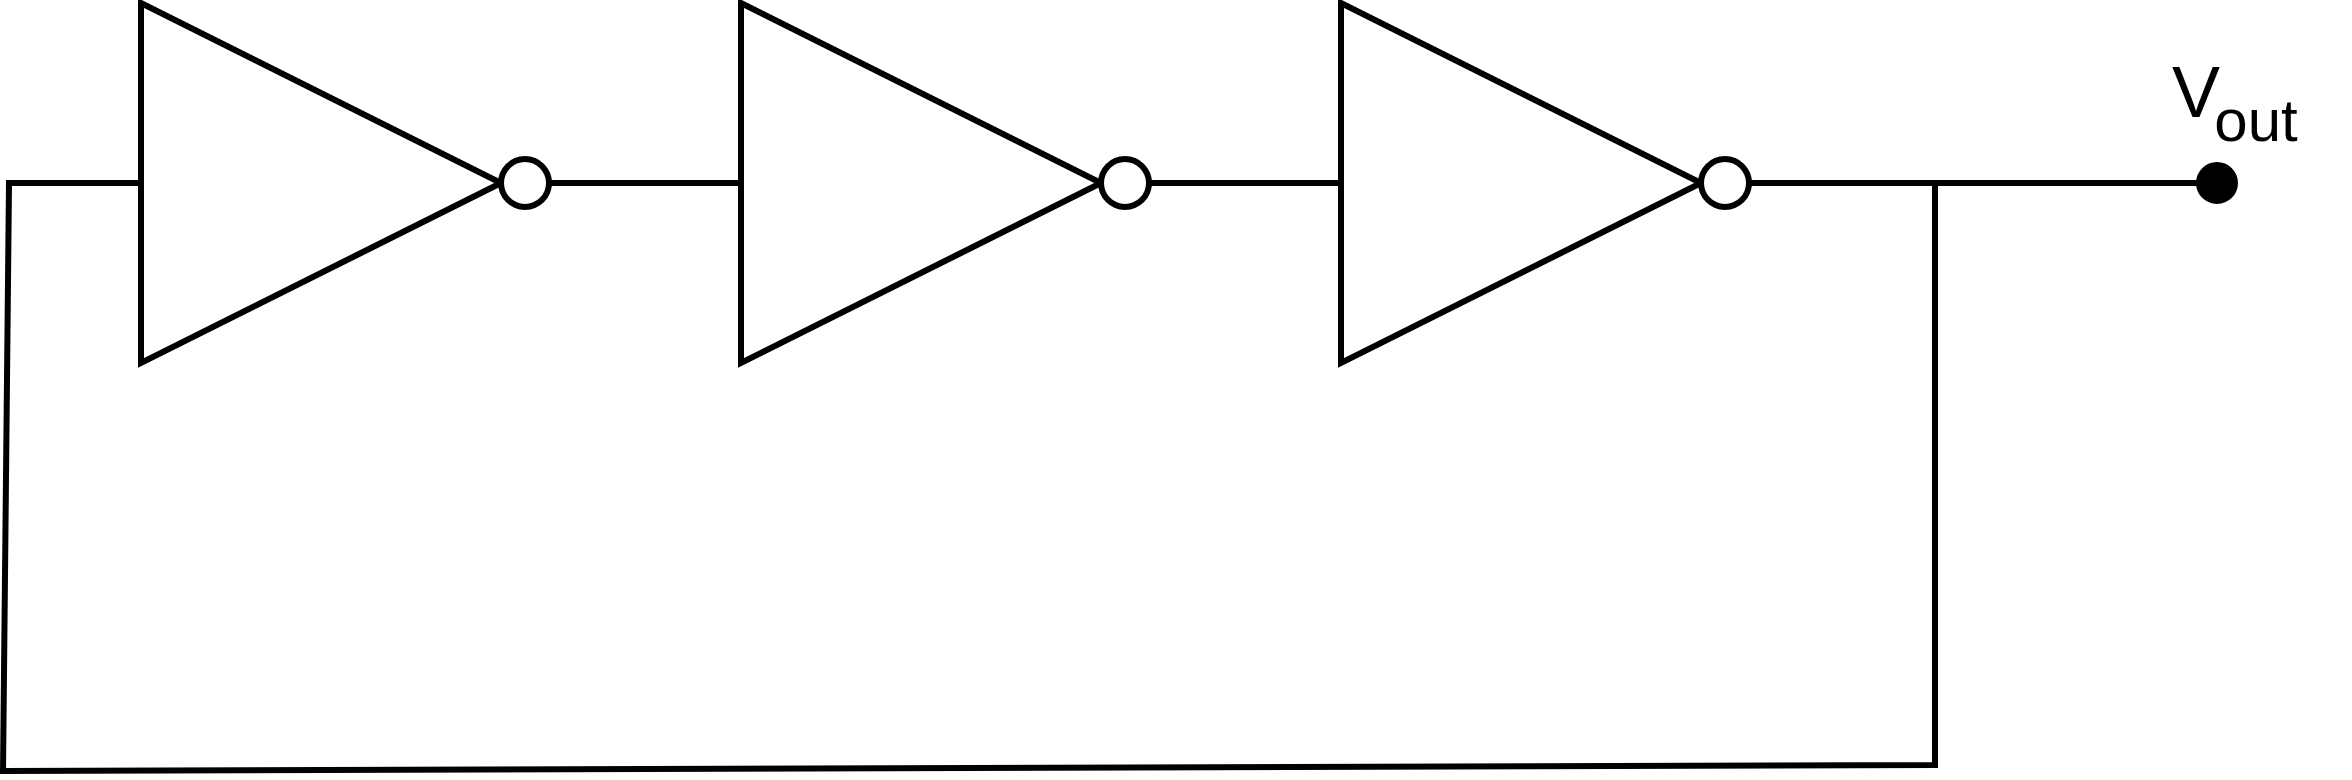
\includegraphics[width=0.6\linewidth]{immagini/ring-oscillator/ring-oscillator-schematico.png}
	\caption{Schematico ring oscillator.}
	\label{fig:ring-oscillator-schematico}
\end{figure}

Questo circuito può generare segnali fino $6\,\mathrm{MHz}$, ma essendo a frequenze così elevate il segnale in uscita non risulta essere un'onda quadta figura \ref{fig:a-oscillatore-ring-oscillator}. Per migliorarne la forma si inserisce in cascata all'uscita due inverter, come in figura \ref{fig:ring-oscillator-schematico-miglirato}, il segnale ricavato si trova a figura \ref{fig:b-oscillatore-ring-oscillator}.

\begin{figure}[h]
	\centering
	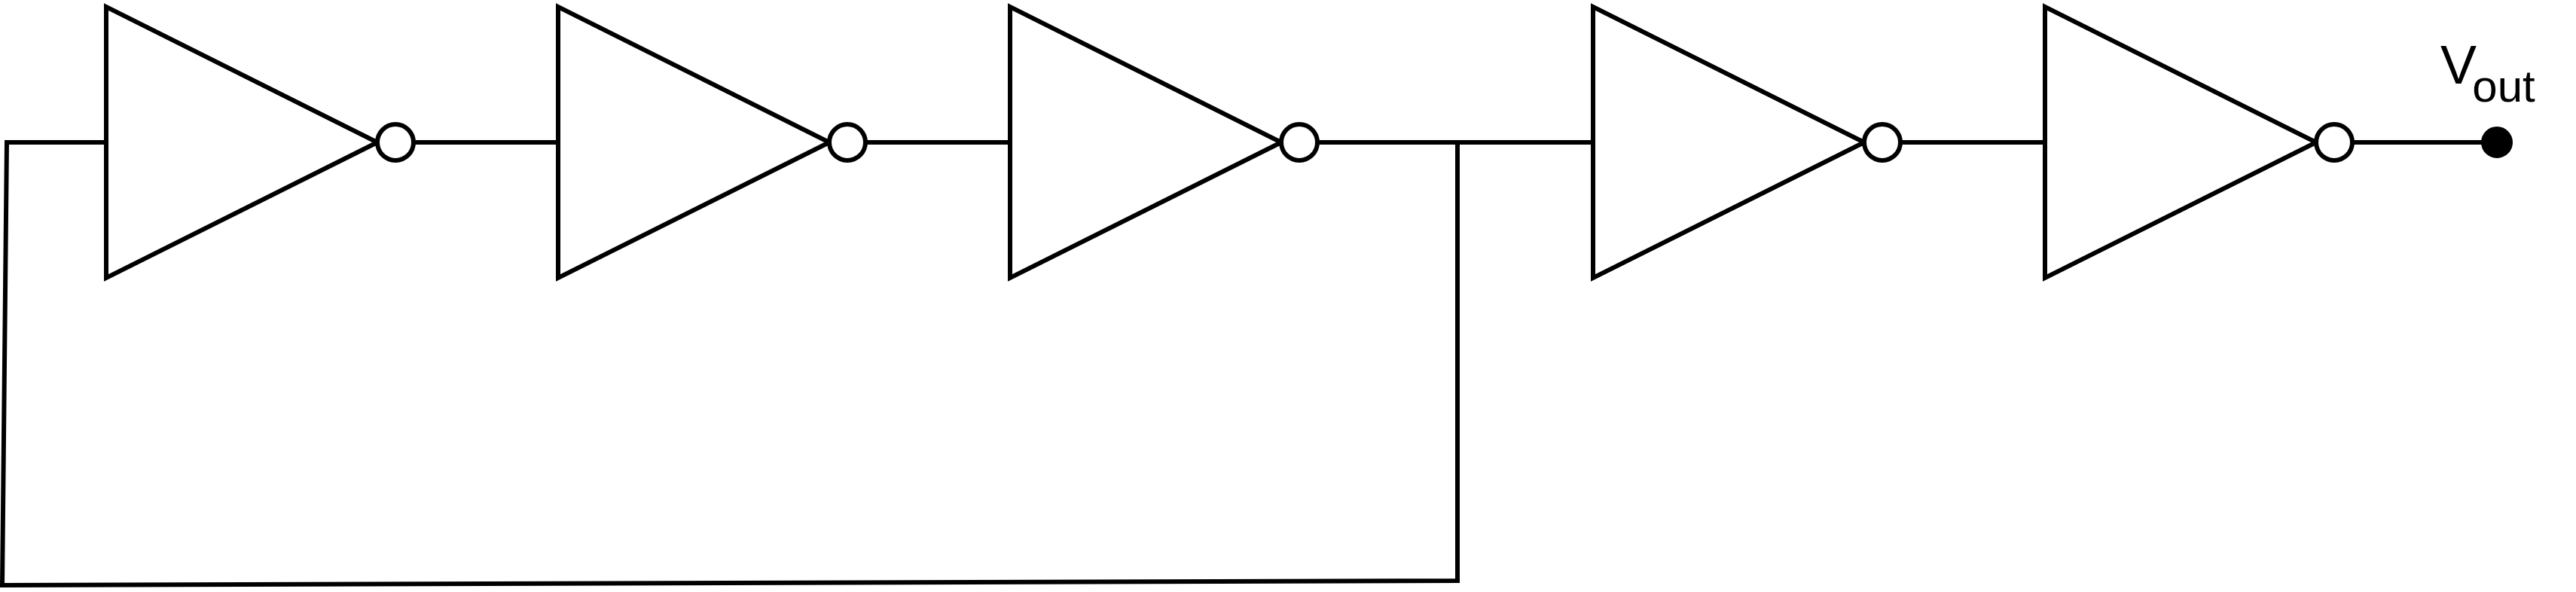
\includegraphics[width=0.7\linewidth]{immagini/ring-oscillator/3InverterNoRes.png}
	\caption{Schematico del ring oscillator con miglioramento del segnale d'uscita.}
	\label{fig:ring-oscillator-schematico-miglirato}
\end{figure}

\begin{figure}[h]
	\centering
	\begin{subfigure}{0.45\linewidth}
		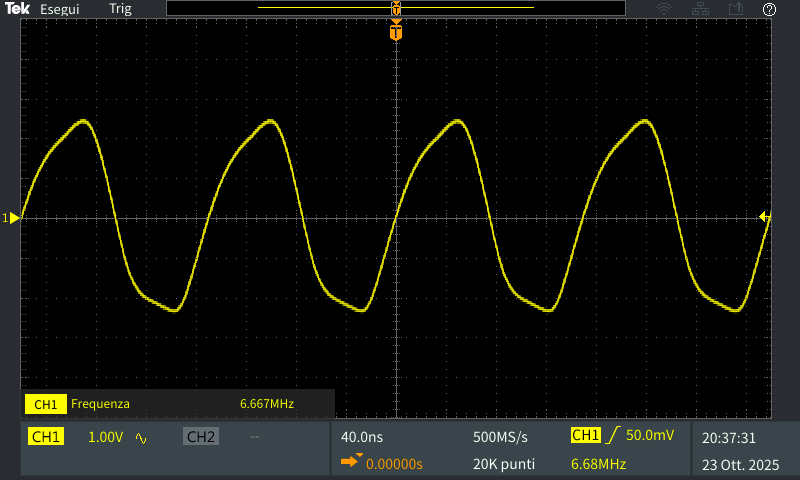
\includegraphics[width = \linewidth]{immagini/ring-oscillator/ring-oscillator-oscillatore.png}
		\caption{Segnale in uscita dallo stadio del ring oscillator.}
		\label{fig:a-oscillatore-ring-oscillator}
	\end{subfigure}
	\quad
	\begin{subfigure}{0.45\linewidth}
		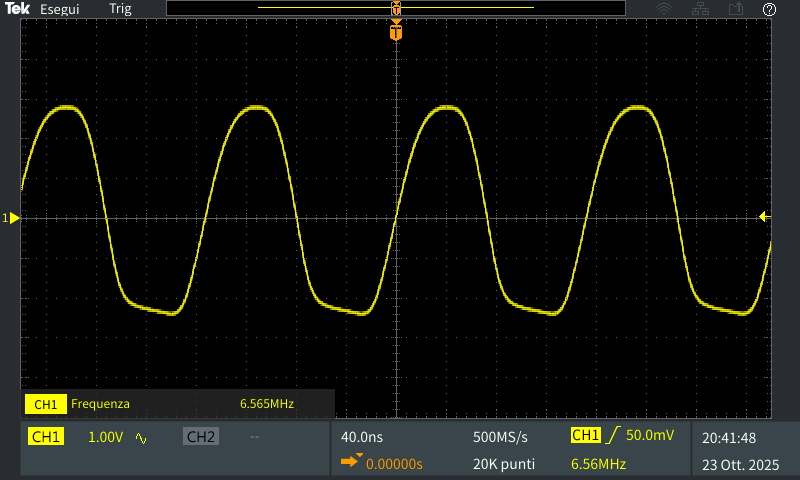
\includegraphics[width = \linewidth]{immagini/ring-oscillator/ring-oscillator-uscita-doppio-inverter-oscillatore.png}
		\caption{Segnale in uscita dallo stadio del ring oscillator.}
		\label{fig:b-oscillatore-ring-oscillator}
	\end{subfigure}
	\caption{Segnali generati dal ring oscillator.}
	\label{fig:oscillatore-ring-oscillator}
\end{figure}

Per poter modificare la frequenza di oscillazione si può utilizzare il circuito a figura \ref{fig:ring-oscillator-schematico-freq} 

\begin{figure}[h]
	\centering
	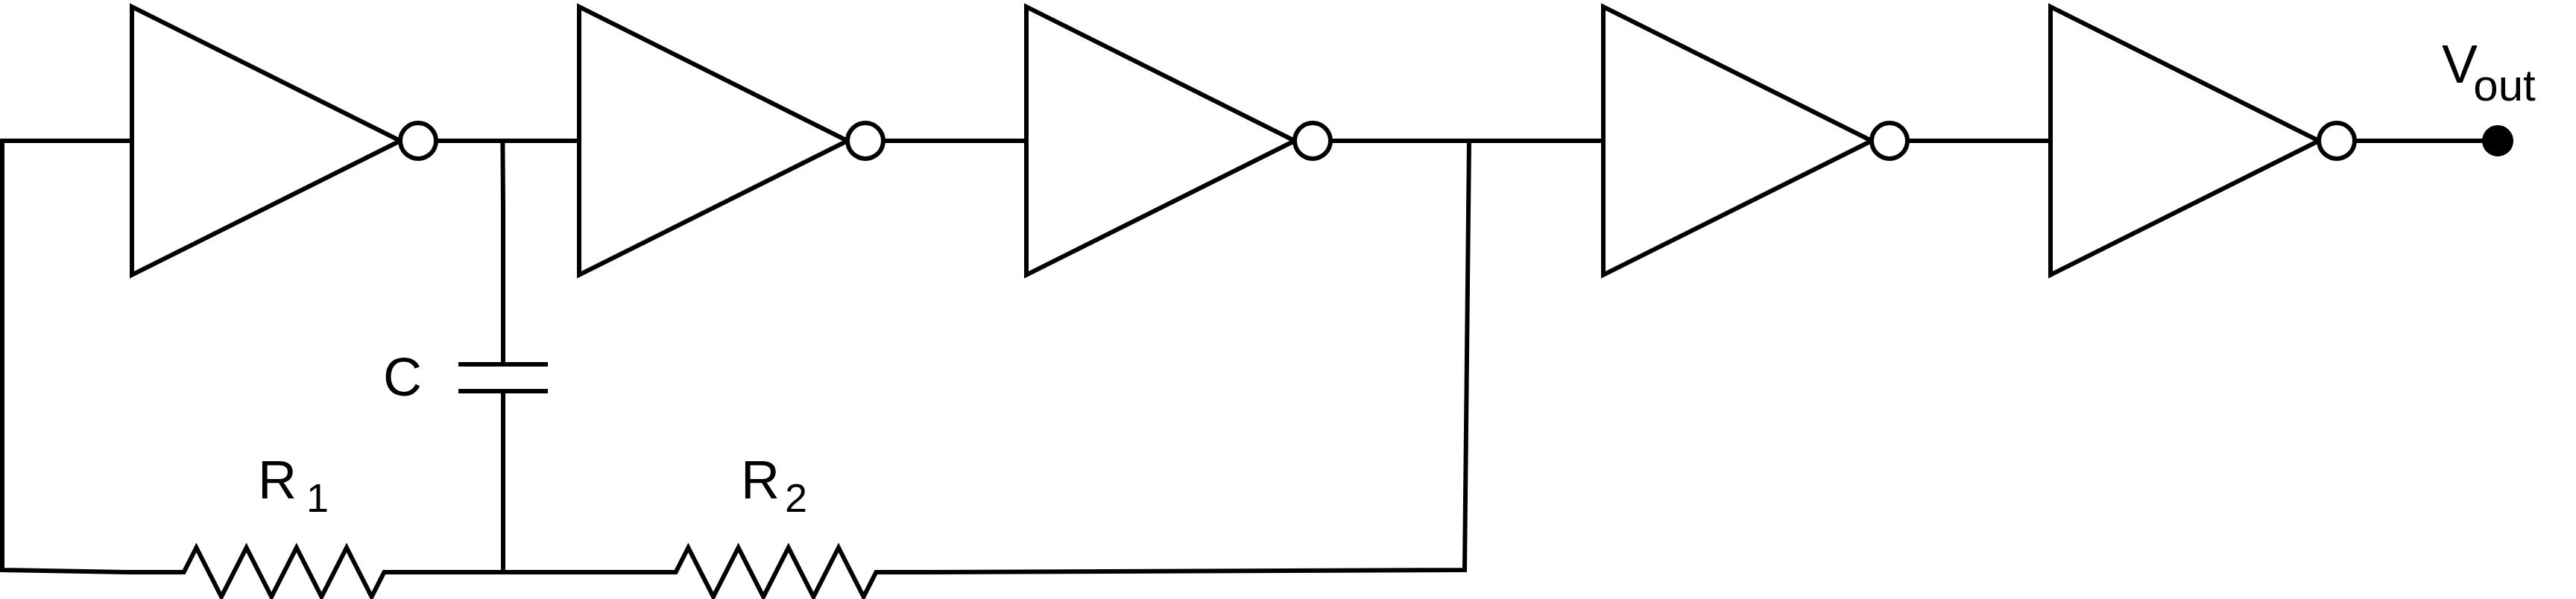
\includegraphics[width=0.7\linewidth]{immagini/ring-oscillator/3InverteRes.png}
	\caption{Schematico del ring oscillator con modifica di frequenza.}
	\label{fig:ring-oscillator-schematico-freq}
\end{figure}

\end{document}

